\chapter{Realizacja projektu}
Niniejszy rozdział omówi architekturę i sposób implementacji projektu KubeFold.


\section{Koncepcja platformy KubeFold}
KubeFold to oprogramowanie, które działa na platformie Kubernetes w trybie Operatora.
Projekt składa się z następujących komponentów:
\begin{itemize}
    \item Operator Kubernetes (z ang. \textit{operator}) - komponent, który zarządzania logiką biznesową.
    Dba o poprawne uruchamianie i zarządzanie podami służącymi do pobierania baz danych białek oraz obliczeń.
    Komponent został dokładnie opisany w sekcji~\ref{subsec:component-operator}.
    \item Komponent pobierania (z ang. \textit{downloader}) - służy do kontroli procesu pobierania i dekompresji baz danych białek.
    Dokładny opis znajduje się w sekcji~\ref{subsec:component-downloader}.
    \item Komponent zarządzający obliczeniami (z ang. \textit{manager}) - obsługuje dodatkowe działania wokół obliczeń takie jak wysyłka artefaktów bądź wysyłanie powiadomienia.
    Opisany został w sekcji~\ref{subsec:component-manager}.
\end{itemize}

%TODO(matisiekpl): verify translation of CRD
Oprócz tego KubeFold wprowadza dwie CRD (\textit{custom resource definition}). Pierwszą z nich jest zasób \textit{ProteinDatabase}.
Reprezentuje on pojedynczą instalację bazy danych białek w klastrze.
Przykładowy kod zasobu jest przedstawiony na listingu~\ref{lst:protein_database}.
W specyfikacji zasobów użytkownik może wybrać jakie bazy danych powinny zostać zainstalowane.
Co więcej, może też wskazać, jaką StorageClasse powinien przyjąć wolumen, służący do przechowywania danych.
Dzięki temu możliwe jest wskazanie klasy, która odpowiada za system plików Lustre (szerzej opisany w sekcji~\ref{subsec:lustre-volumes}).
W przykładowym kodzie wskazano klasę o nazwie \textit{fsx-sc}, która podpina się pod wolumeny AWS FSx for Lustre (zobacz~\ref{subsec:amazon-fsx-for-lustre}).
Z perspektywy użytkownika ten zasób może być zarządzany przez \texttt{kubectl} co zostało pokazane na grafice~\ref{fig:proteindatabase_terminal}.

\begin{lstlisting}[language=yaml,caption={Przykładowy kod YAML zasobu ProteinDatabase},label={lst:protein_database}]
apiVersion: data.kubefold.io/v1
kind: ProteinDatabase
metadata:
  name: proteindatabase-sample
spec:
  datasets:
    bfd: true
    mgyclusters: true
    nt: true
    pdb: true
    pdbseqreq: true
    rfam: true
    rnacentral: true
    uniref90: true
    uniprot: true
  volume:
    storageClassName: fsx-sc
\end{lstlisting}

\begin{figure}[htbp]
    \centering
    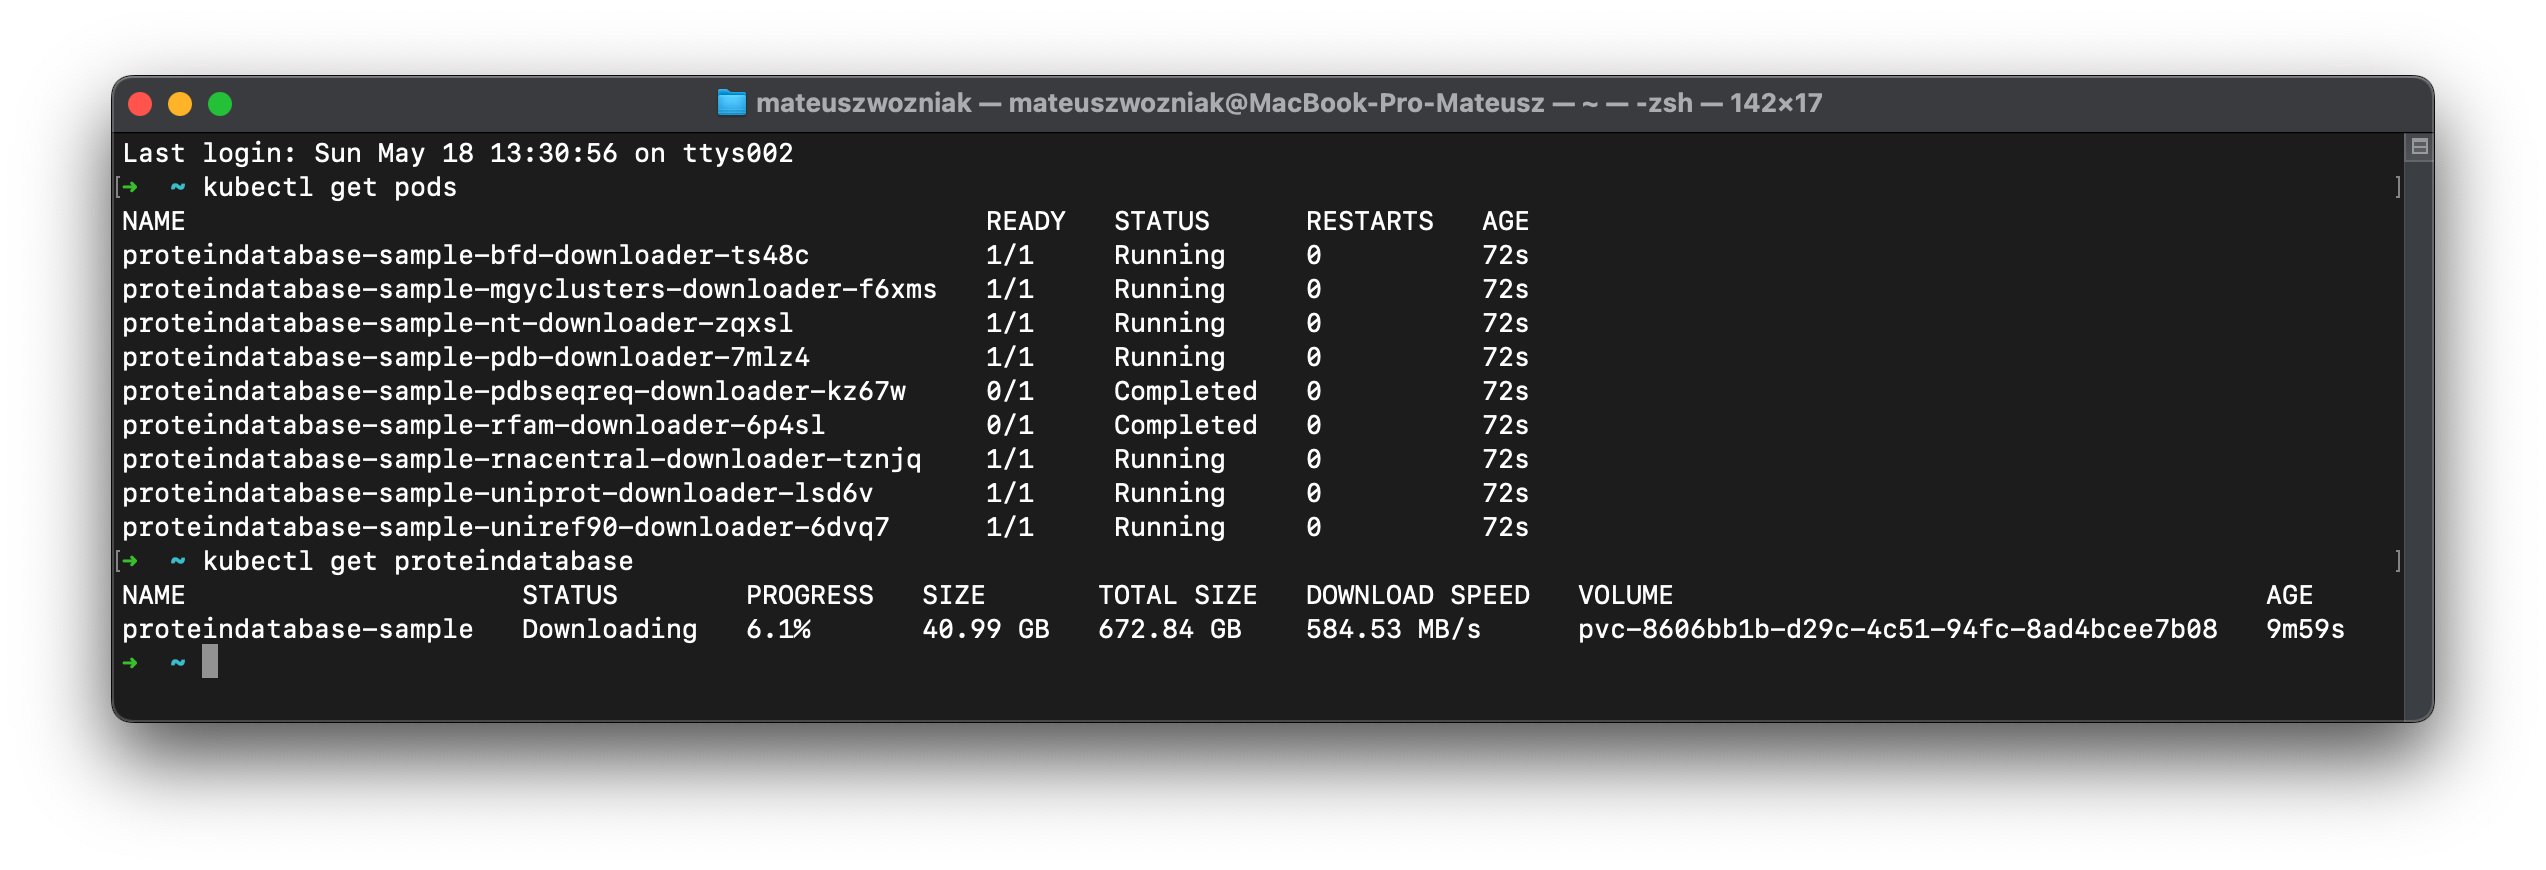
\includegraphics[width=\textwidth]{images/proteindatabase_terminal}
    \caption{Terminal output presenting \textit{ProteinDatabase} resource}
    \label{fig:proteindatabase_terminal}
\end{figure}

Ponadto KubeFold obsługuje definicję zasobu \textit{ProteinConformationPrediction}.
Odpowiada on za pojedyncze obliczenie konformacji białka na podstawie dostarczonej sekwencji aminokwasów.
Przykład definicji jest przedstawiony na listingu~\ref{lst:protein_conformation_prediction}.
Użytkownik może wskazać ustawienia zadania takie jak:
\begin{itemize}
    \item bazę danych białek, na podstawie której algorytm AlphaFold ma przeprowadzić przeszukiwanie
    \item sekwencję aminokwasów w postaci ciągu liter
    \item ustawienia wolumenu służącego do przechowywania tymczasowych plików obliczenia
    \item wskazanie źródła pliku wag modelu AlphaFold.
    W przykładowym kodzie ustawiono źródło jako zdalny serwer HTTP.
    \item docelową lokalizację artefaktów.
    W aktualnej wersji projektu KubeFold wspierany jest jedynie system składowania obiektów AWS S3 (zobacz.~\ref{subsec:amazon-s3-object-storage}).
    \item opcje powiadamiania użytkownika.
    Przykładowy kod ma ustawione pojedyczne powiadomienie SMS na numer telefonu.
\end{itemize}
Zarządzanie może odbywać się przez \texttt{kubectl} co zostało pokazane na grafice~\ref{fig:proteinconformationprediction_terminal}.

\begin{figure}[htbp]
    \centering
    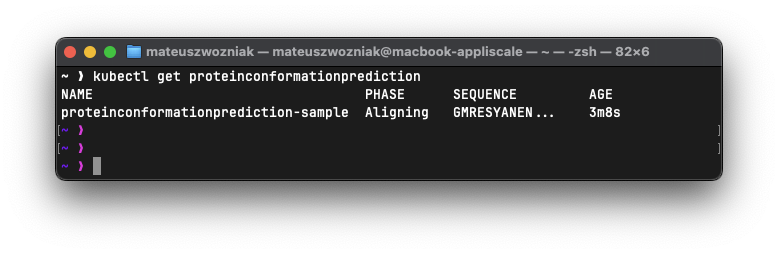
\includegraphics[width=\textwidth]{images/proteinconformationprediction_terminal}
    \caption{Terminal output presenting \textit{ProteinConformationPrediction} resource}
    \label{fig:proteinconformationprediction_terminal}
\end{figure}

\begin{lstlisting}[language=yaml,caption={Przykładowy kod YAML zasobu ProteinConformationPrediction},label={lst:protein_conformation_prediction}]
apiVersion: data.kubefold.io/v1
kind: ProteinConformationPrediction
metadata:
  name: proteinconformationprediction-sample
spec:
  database: proteindatabase-sample
  protein:
    id: [ 'A','B' ]
    sequence: GMRESY...LQQANDLKQG
  model:
    volume:
      storageClassName: fsx-sc
    weights:
      http: https://staticfilehosting.com/af3.bin.zst
    seeds:
      - 1
  destination:
    s3:
      bucket: kubefold-artifacts-sample
      region: eu-central-1
  notify:
    region: eu-central-1
    sms:
      - "+48140690323"
\end{lstlisting}


\section{Użyte technologie}
Wszystkie trzy komponenty zostały napisane w języku Go w wersji 1.24 (więcej o nim w sekcji~\ref{subsec:go-programming-language}).
Był to naturalny wybór, ponieważ Go jest de facto standardem w przypadku tworzenia oprogramowania chmurowego.
Kod źródłowy komponentów był archiwizowany w repozytorium Git~\cite{git} w serwisie GitHub~\cite{github}.

W celu kompilacji aplikacji i spakowania plików wykonywalnych do obrazu kontenera użyto standardowego buildera od Dockera.

Dystrybucja obrazów odbywa się za pomocą rejestru Github Container Registry (\textit{ghcr.io})~\cite{ghcr}.
Obrazy są automatycznie budowane przy każdym wypchnięciu tagu Git przez narzędzie GitHub Actions~\cite{github_actions}.
Flow działania zostało przestawione na rys.~\ref{fig:docker-images-flow}.

\begin{figure}[htbp]
    \centering
    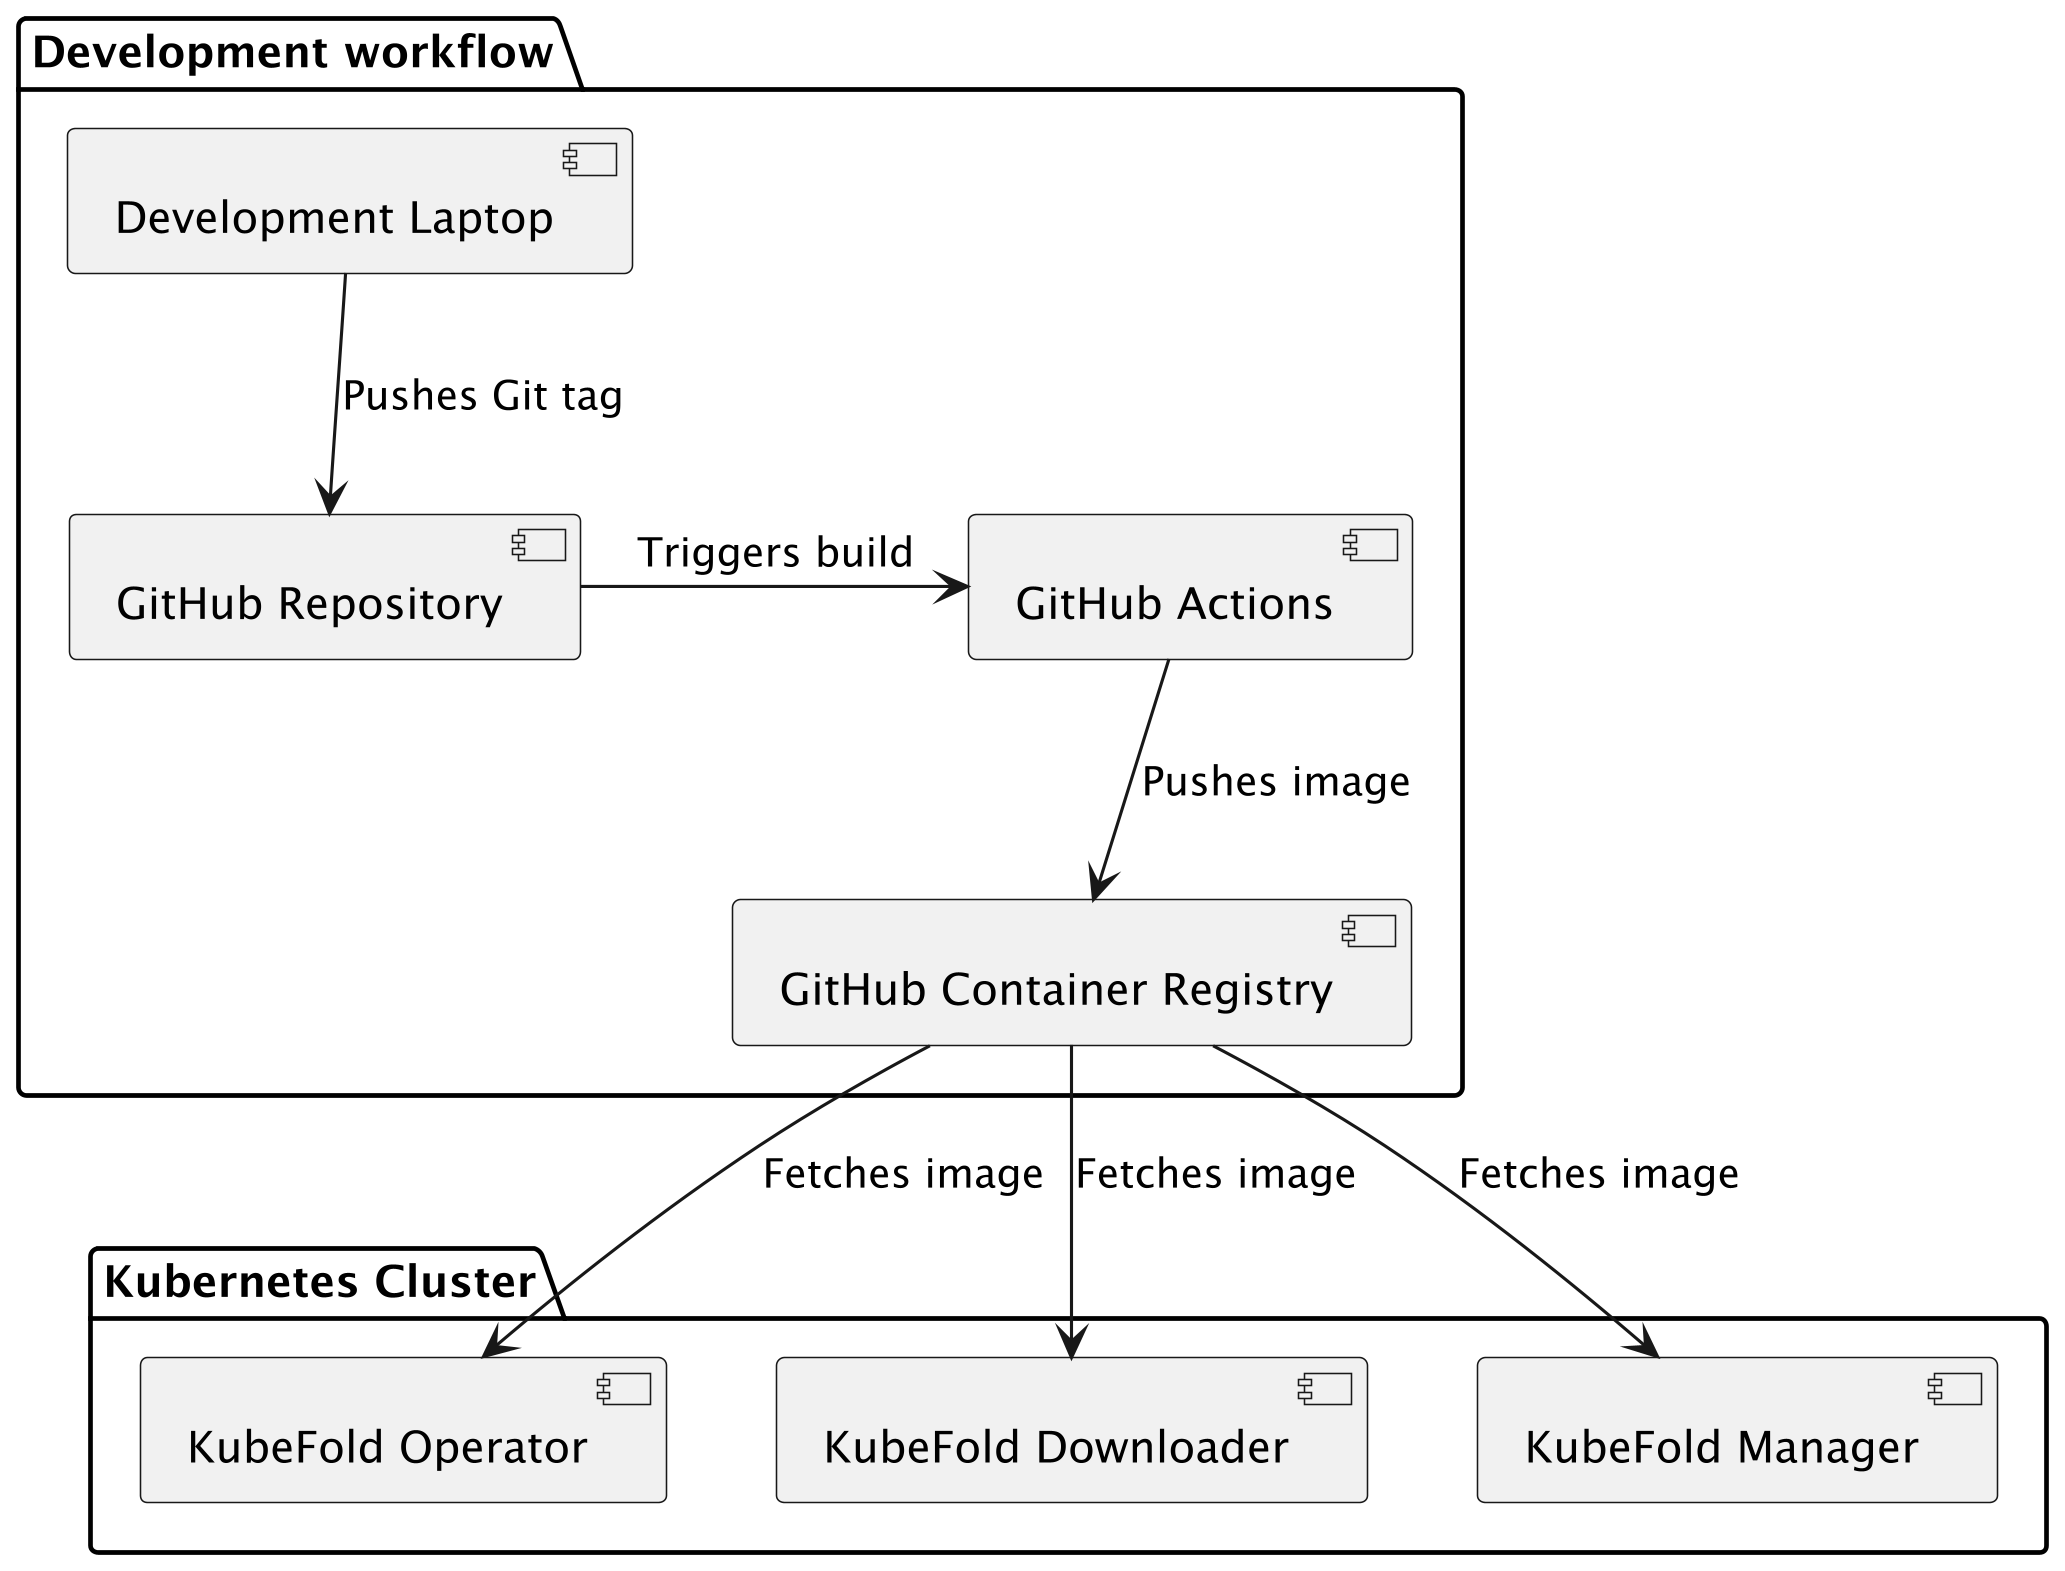
\includegraphics[width=0.8\textwidth]{images/images}
    \caption{Development workflow between GitHub and cluster}
    \label{fig:docker-images-flow}
\end{figure}

Komponent Operatora (szerzej opisany w~\ref{subsec:component-operator}) został utworzony na podstawie framework KubeBuilder~\cite{kubebuilder}.
KubeBuilder to framework, który służy do pisania natywnych operatorów Kubernetes.
Tworzy on strukturę katalogów projektu oraz od razu zapewnia zarządzanie elementami takimi jak:
\begin{itemize}
    \item Elekcja lidera operatora-niektóre instancje operatorów mogą być uruchomione na wielu węzłach klastra jednocześnie, aczkolwiek jeżeli istnieje potrzeba wybrania jednej wyróżnionej instancji, to elekcja lidera wybiera go.
    \item Generowanie skryptów instalacyjnych-KubeBuilder ma możliwość wygenerowania gotowych skryptów instalacyjnych, które mogą później posłużyć do automatycznej instalacji operatora i wszystkich jego zależności w klastrze jednym wykonaniem polecenia \textit{kubectl apply}.
    \item Definicje ról i permisji.
    Kubernetes korzysta z modelu autoryzacji o nazwie \textit{RBAC} (Role-Based Access Control)~\cite{k8s_rbac}.
    KubeBuilder wykrywa jakie permisje powinna mieć instancja operatora i upewnia się, że odpowiednie permisje zostały mu przyznane.
\end{itemize}


\section{Architektura rozwiązania}

Oba wprowadzone zasoby CRD zarządzają pewnymi określonymi podrzędnymi zasobami.

Zasób \textit{ProteinDatabase} tworzy przede wszystkim: persistent volume claim, który będzie składował dane baz danych białek oraz zbiór jobów, które odpowiadają za pobieranie poszczególnych baz.
Architektura zależności zasobów została przedstawiona na diagramie~\ref{fig:proteindatabase}.
Ilość jobów jest dokładnie taka sama jak ilość wybranych baz danych zdefiniowanych w kodzie YAML.
Ze względu na taki rozdział procesu pobierania, możliwe jest, by wiele węzłów pobierało dane niezależne w tym samym czasie.
W takim przypadku sumaryczna przepustowość się zwiększy, ponieważ nie będzie ona ograniczona przez limit prędkości pobierania interfejsu sieciowego pojedynczego węzła.
Wszystkie pody utworzone przez Joby podpinają się do wspólnego wolumenu i przeprowadzają pobieranie baz z serwerów Google, używając protokołu HTTP.
W trakcie pobierania postęp jest na bieżąco logowany do wyjścia \textit{stdout} kontenera.
Dzięki temu operator może odczytywać logi kontenera i na bieżąco śledzić postęp.
Pody jak i wolumen są dowiązane do zasobu \textit{ProteinDatabase} za pomocą mechanizmu \textit{ownerReferences}.
W przypadku usunięcia nadrzędnego zasobu, zasoby podrzędne również zostaną automatycznie usunięte.
Funkcjonalność automatycznego czyszczenia zasobów podrzędnych jest zrealizowana w implementacji Kubernetesa, a nie operatora.

\begin{figure}[htbp]
    \centering
    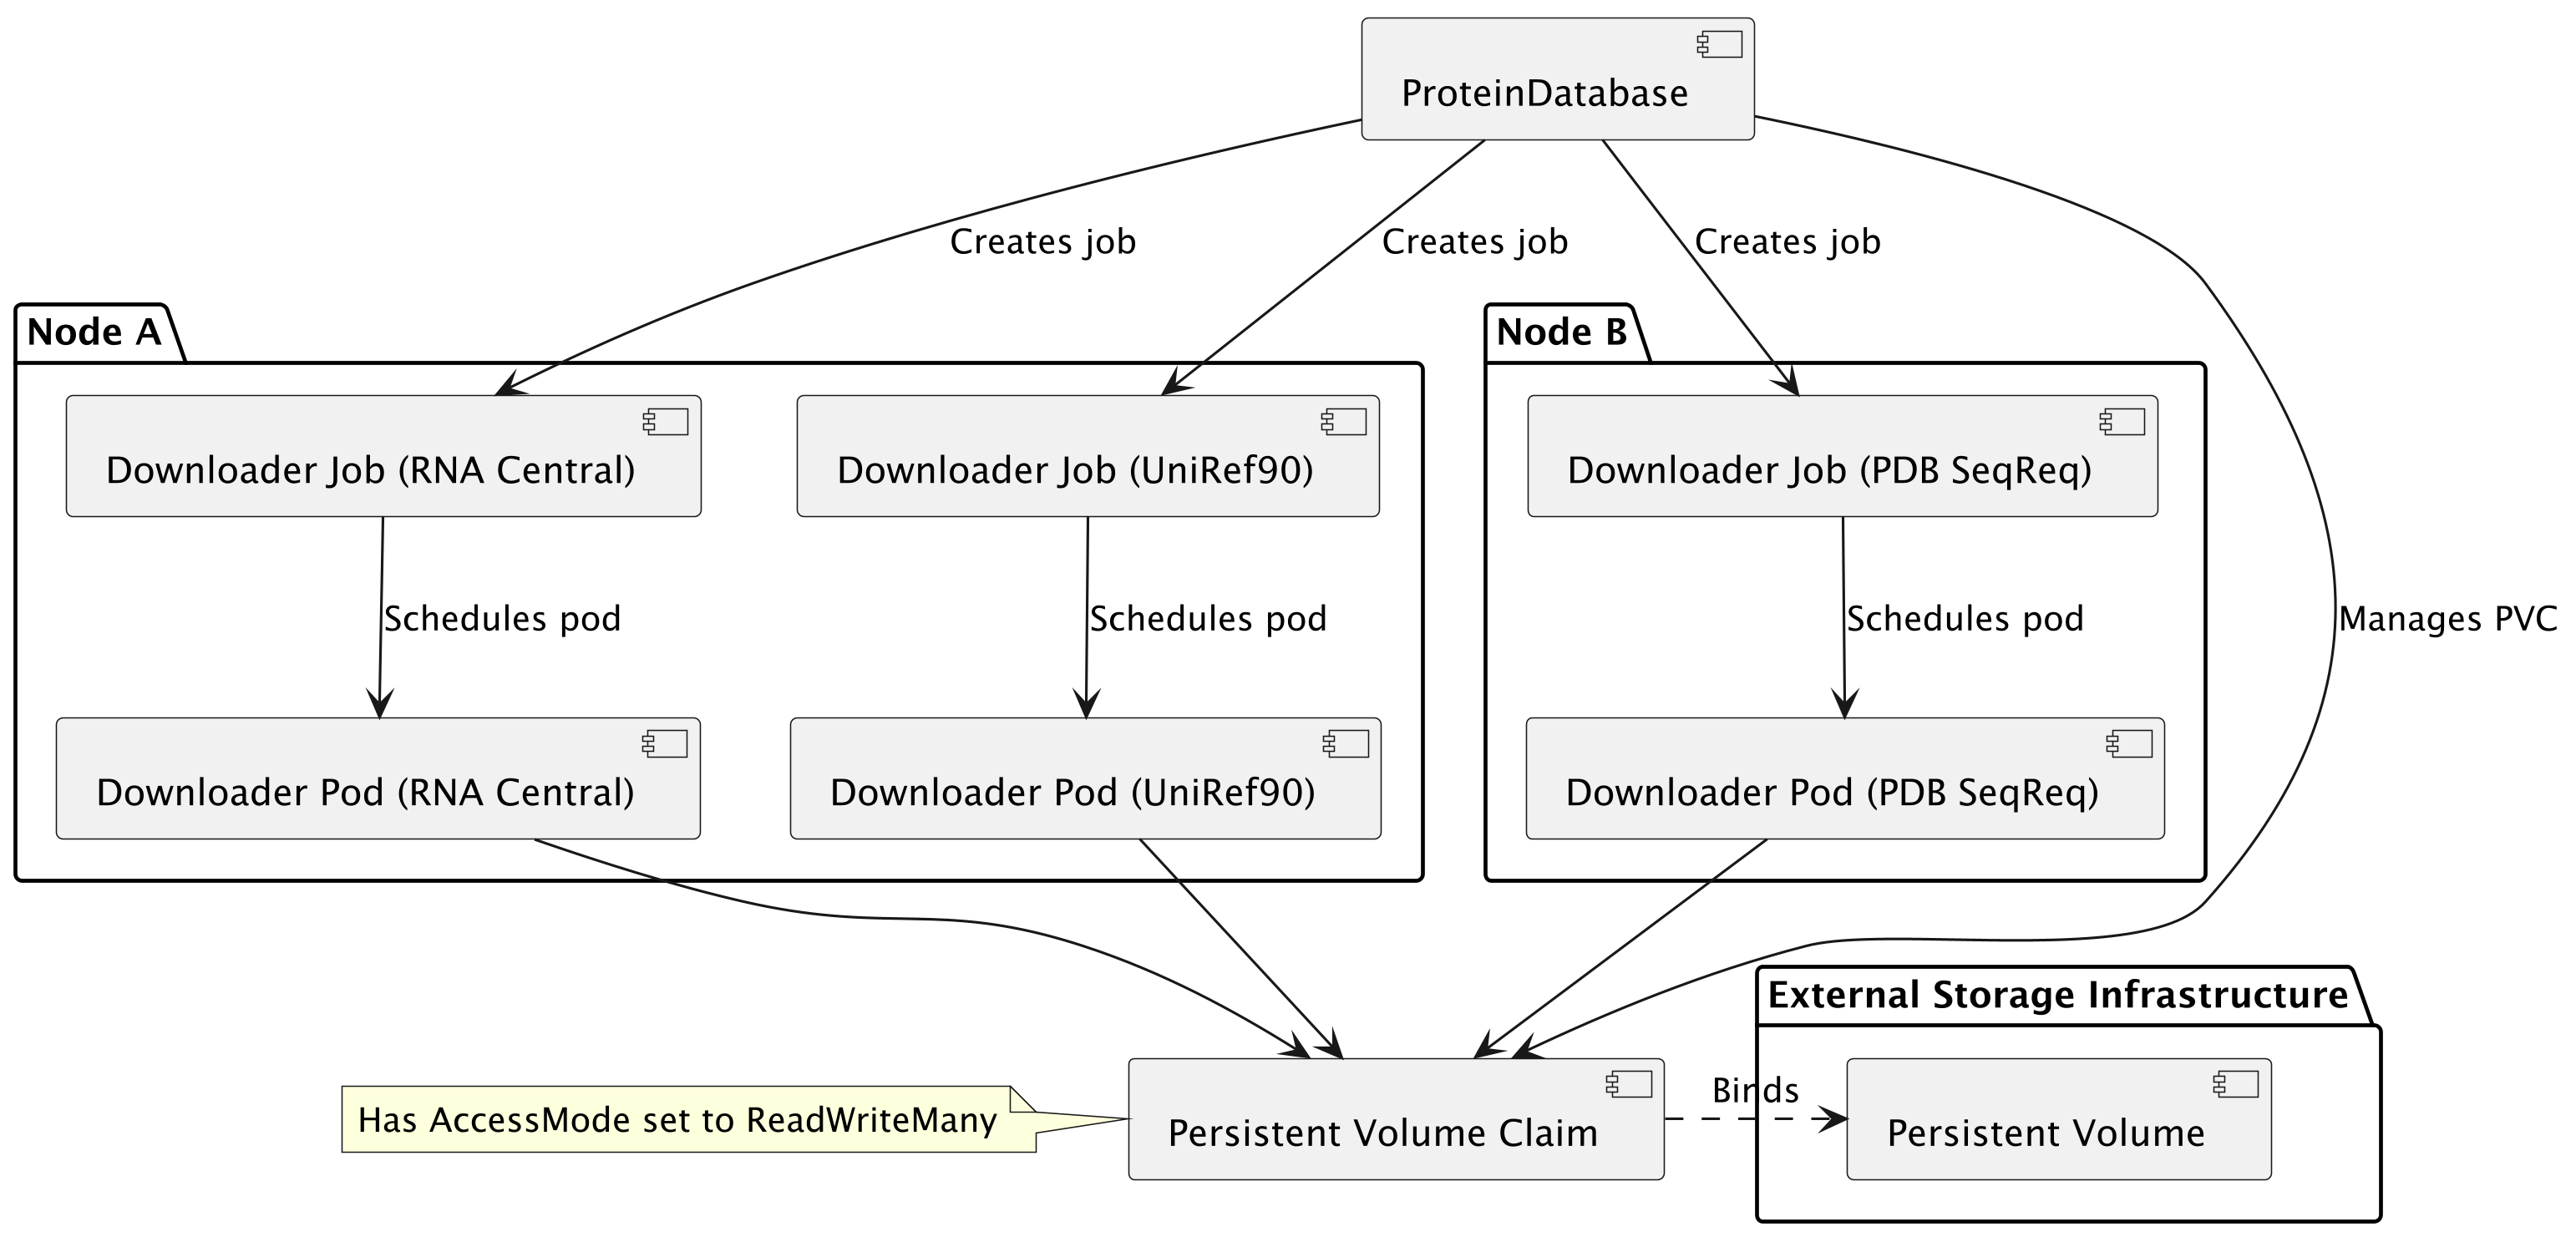
\includegraphics[width=\textwidth]{images/proteindatabase}
    \caption{Cluster resource architecture of ProteinDatabase}
    \label{fig:proteindatabase}
\end{figure}

\begin{figure}[htbp]
    \centering
    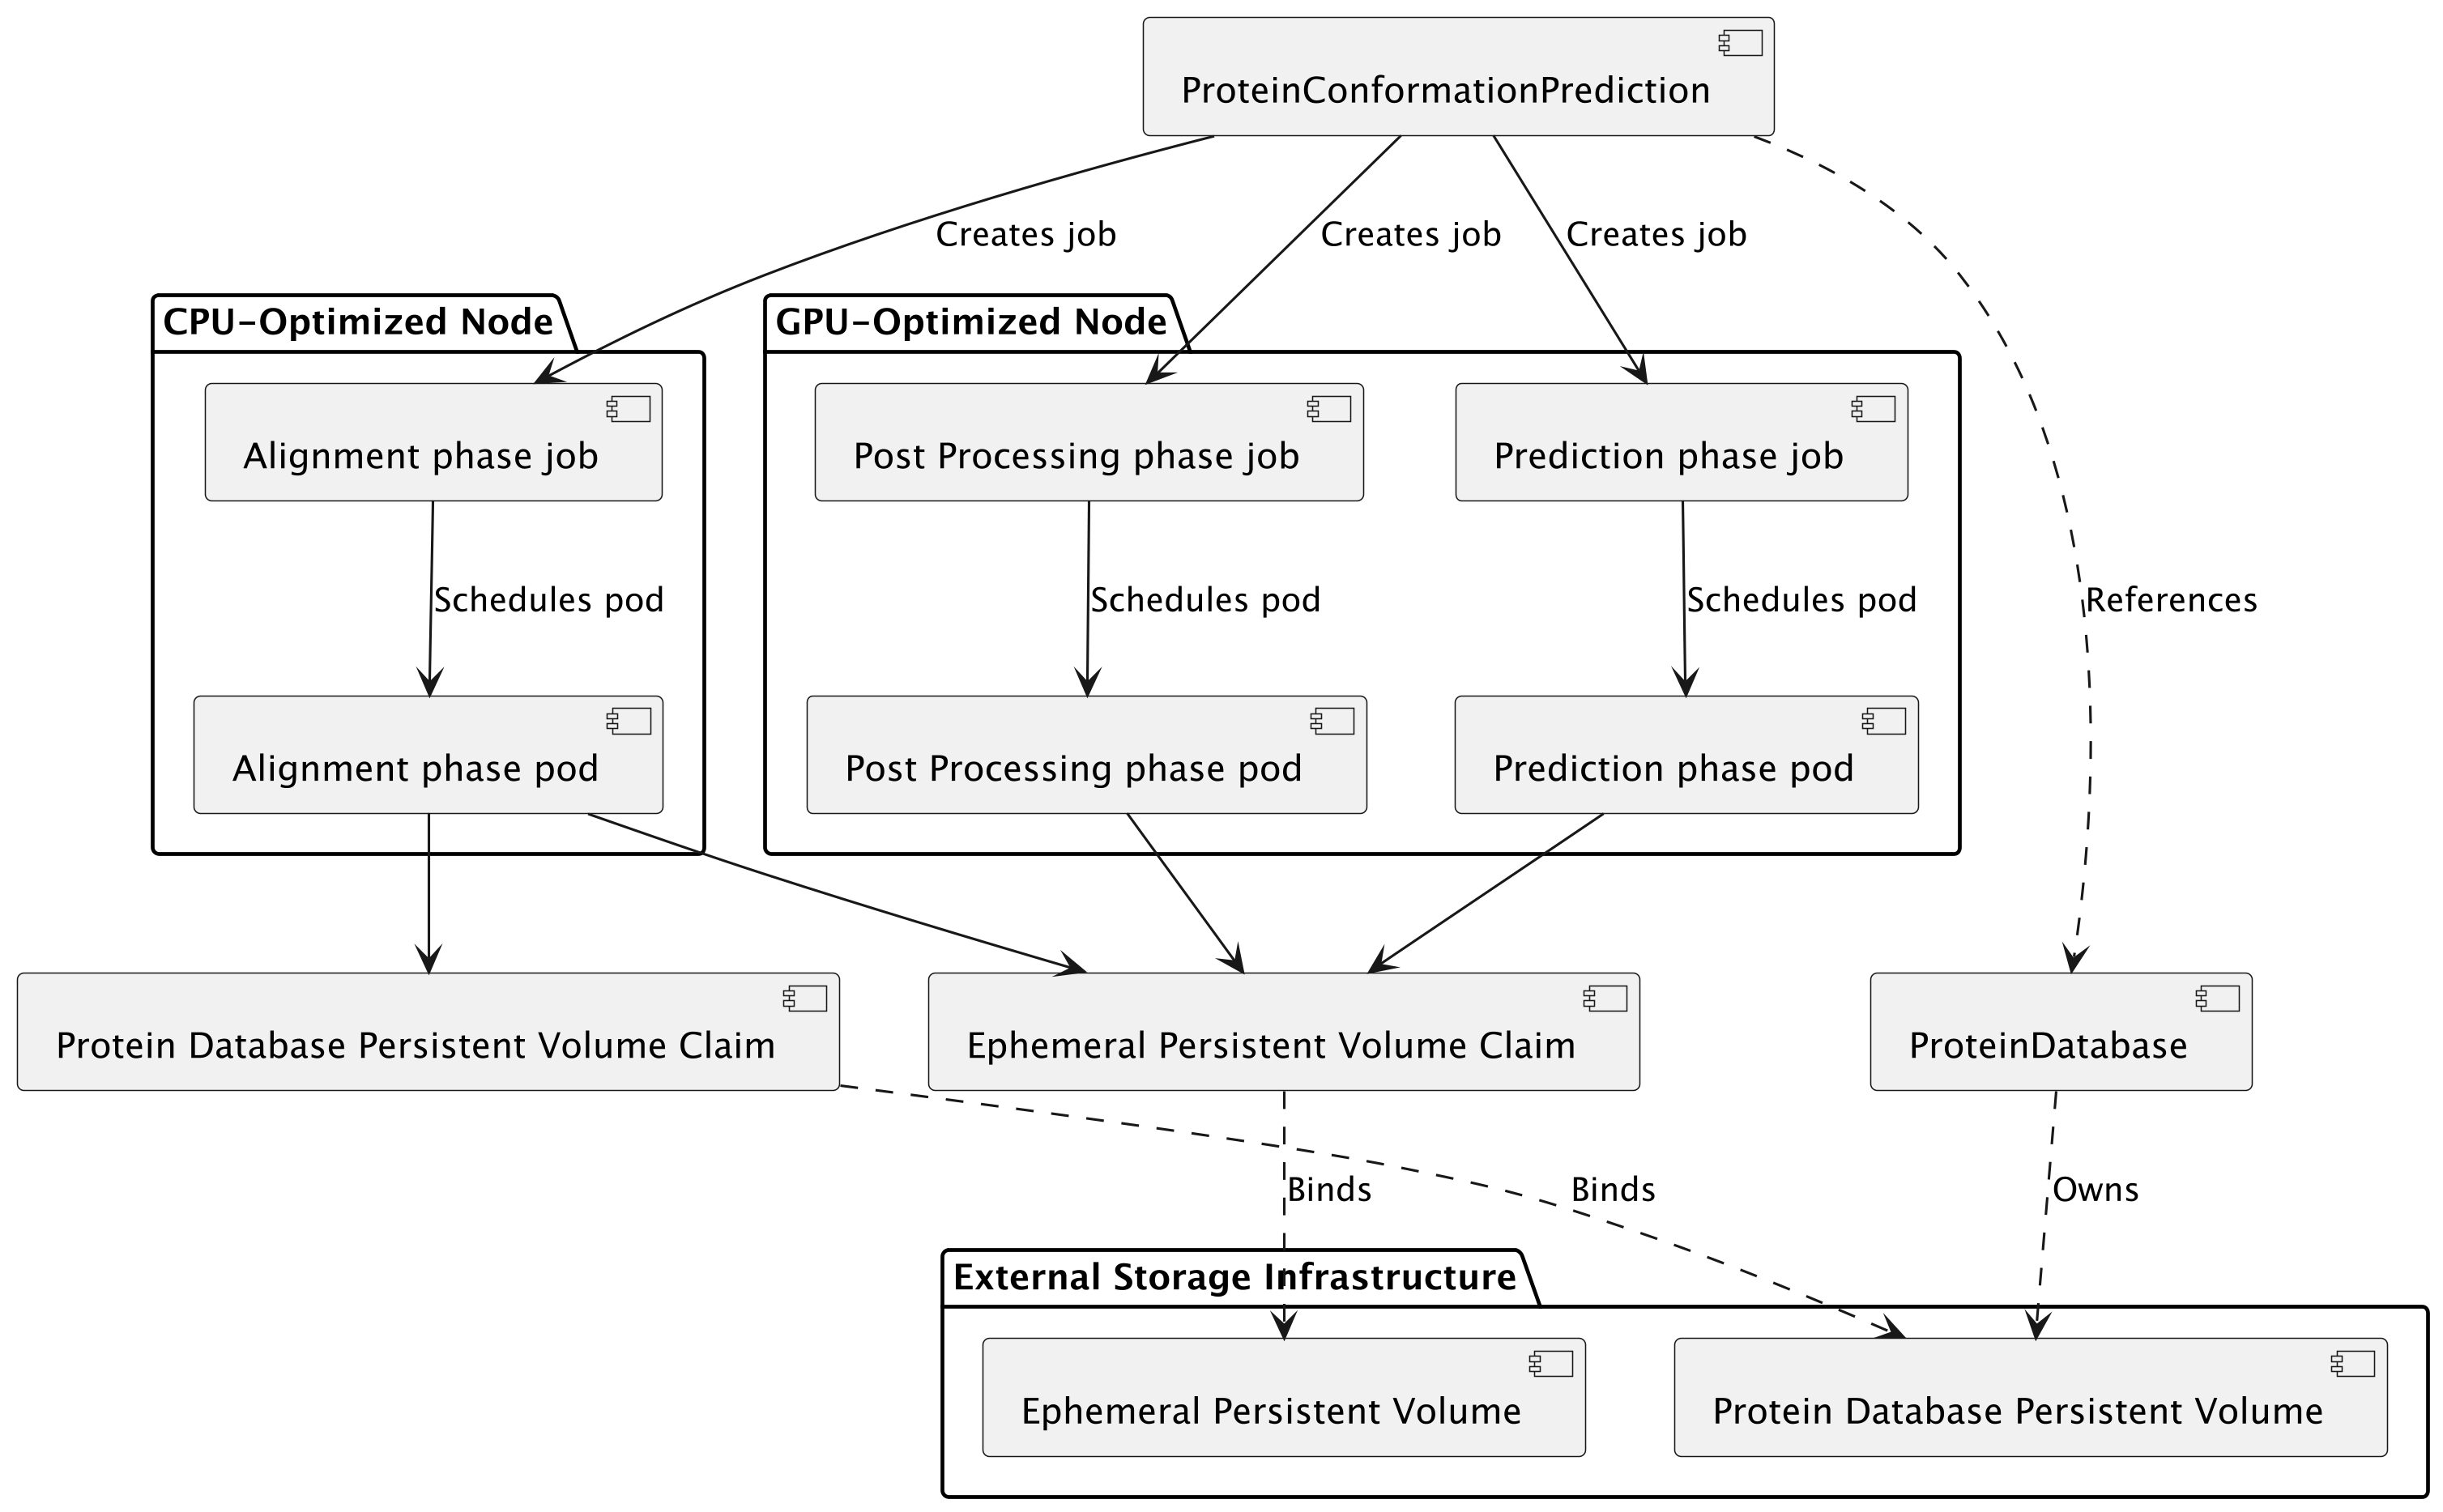
\includegraphics[width=\textwidth]{images/proteinconformationprediction}
    \caption{Cluster resource architecture of ProteinConformationPrediction}
    \label{fig:proteinconformationprediction}
\end{figure}

z kolei zasób \textit{ProteinConformationPrediction} zarządza trzema Jobami.
\begin{itemize}
    \item Faza Alignmentu.
    W tej fazie AlphaFold przeszukuje istniejące bazy danych białek w celu znalezienia dopasowań.
    Ta faza odbywa się w podzie schedulowanych na instancjach zoptymalizowanych pod względem CPU. Pod używa obrazu AlphaFold.
    \item Faza Predykcji.
    Faza, w której algorytm dokonuje faktycznej predykcji trójwymiarowej struktury białka.
    W tej fazie pody są scheduowane na instancjach wyposażonych w akceleratory obliczeń tensorowych.
    Pod również używa obrazu AlphaFold.
    \item Faza Post Processingu.
    Ta faza odpowiada za wysłanie artefaktów do docelowego magazynu danych oraz ewentualne wysłanie powiadomień do członków zespołu badawczego.
    Pod używa obrazu komponentu Managera.
\end{itemize}

Zatem na każde wystąpienie zasobu \textit{ProteinConformationPrediction} przypadają dokładnie trzy Joby i trzy pody.
Oprócz tego \textit{ProteinConformationPrediction} tworzy PersistentVolumeClaim na dane tymczasowe.
W tym wolumenie są składowane wyniki fazy Alignment oraz potencjalnie znalezione struktury białka.

Podobnie jak w przypadku \textit{ProteinDatabase} zasoby są ze sobą spięte mechanizmem \textit{ownerReferences}.
Architektura zależności zasobów została przedstawiona na diagramie~\ref{fig:proteinconformationprediction}.


\section{Opis komponentów}

\subsection{Komponent operatora}\label{subsec:component-operator}
\textit{Repozytorium kodu: \url{https://github.com/kubefold/operator}}

Główny komponent platformy KubeFold napisany w języku Go.
Operator jest instalowany na klastrze Kubernetes jako zasób Deployment i podpina się on do API Servera Kubernetesa używając do tego odpowiedniej ClusterRole.
Dzięki temu ma on dostęp do interakcji z interfejsem REST API, który umożliwia zarządzanie zasobami utworzonymi w ramach klastra.

Najważniejszymi elementami operatora KubeFold są dwa tak zwane kontrolery, odpowiadające za reconciling dwóch definicji CRD wprowadzonych w ramach projektu.
Każdy operator klastra działa na wzór pętli kontroli-nieskończona pętla stale monitoruje zmiany oczekiwanych stanów zasobów w klastrze i koryguje stan faktyczny by był jak najbardziej zgodny z zadanym.
W przypadku operatora KubeFold pętla kontroli działa jedynie na jednej, wyróżnionej instancji operatora.
O tym, która uruchomiona instancja zostanie wyróżniona, decyduje system elekcji dostarczony przez narzędzie KubeBuilder.

Pierwszy kontroler recounciluje stan zasobu \textit{ProteinDatabase}.
W przypadku wykrycia pojawienia się nowego zasobu tego typu wykonuje następujące operacje:
\begin{enumerate}
    \item Tworzy nowy PersistentVolumeClaim i ustawia parametr storageClassName.
    \item Gdy PersistentVolumeClaim zostanie zbindowany do konkretnego wolumenu, tworzy kilka Jobów odpowiadających za pobieranie poszczególnych baz danych.
    Każdy pod ma zamountowany PersistentVolumeClaim.
    \item Uruchamia obserwator logów-osobny wątek, który stale monitoruje stan Jobów, Podów oraz odczytuje z nich logi.
    Dzięki logom jest w stanie dynamicznie aktualizować status \textit{ProteinDatabase} informując użytkownika o postępie pobierania, a także przepustowości łącza.
\end{enumerate}
Operacje te zostały przedstawione na diagramie~\ref{fig:proteindatabase_controller}.

\begin{figure}[htbp]
    \centering
    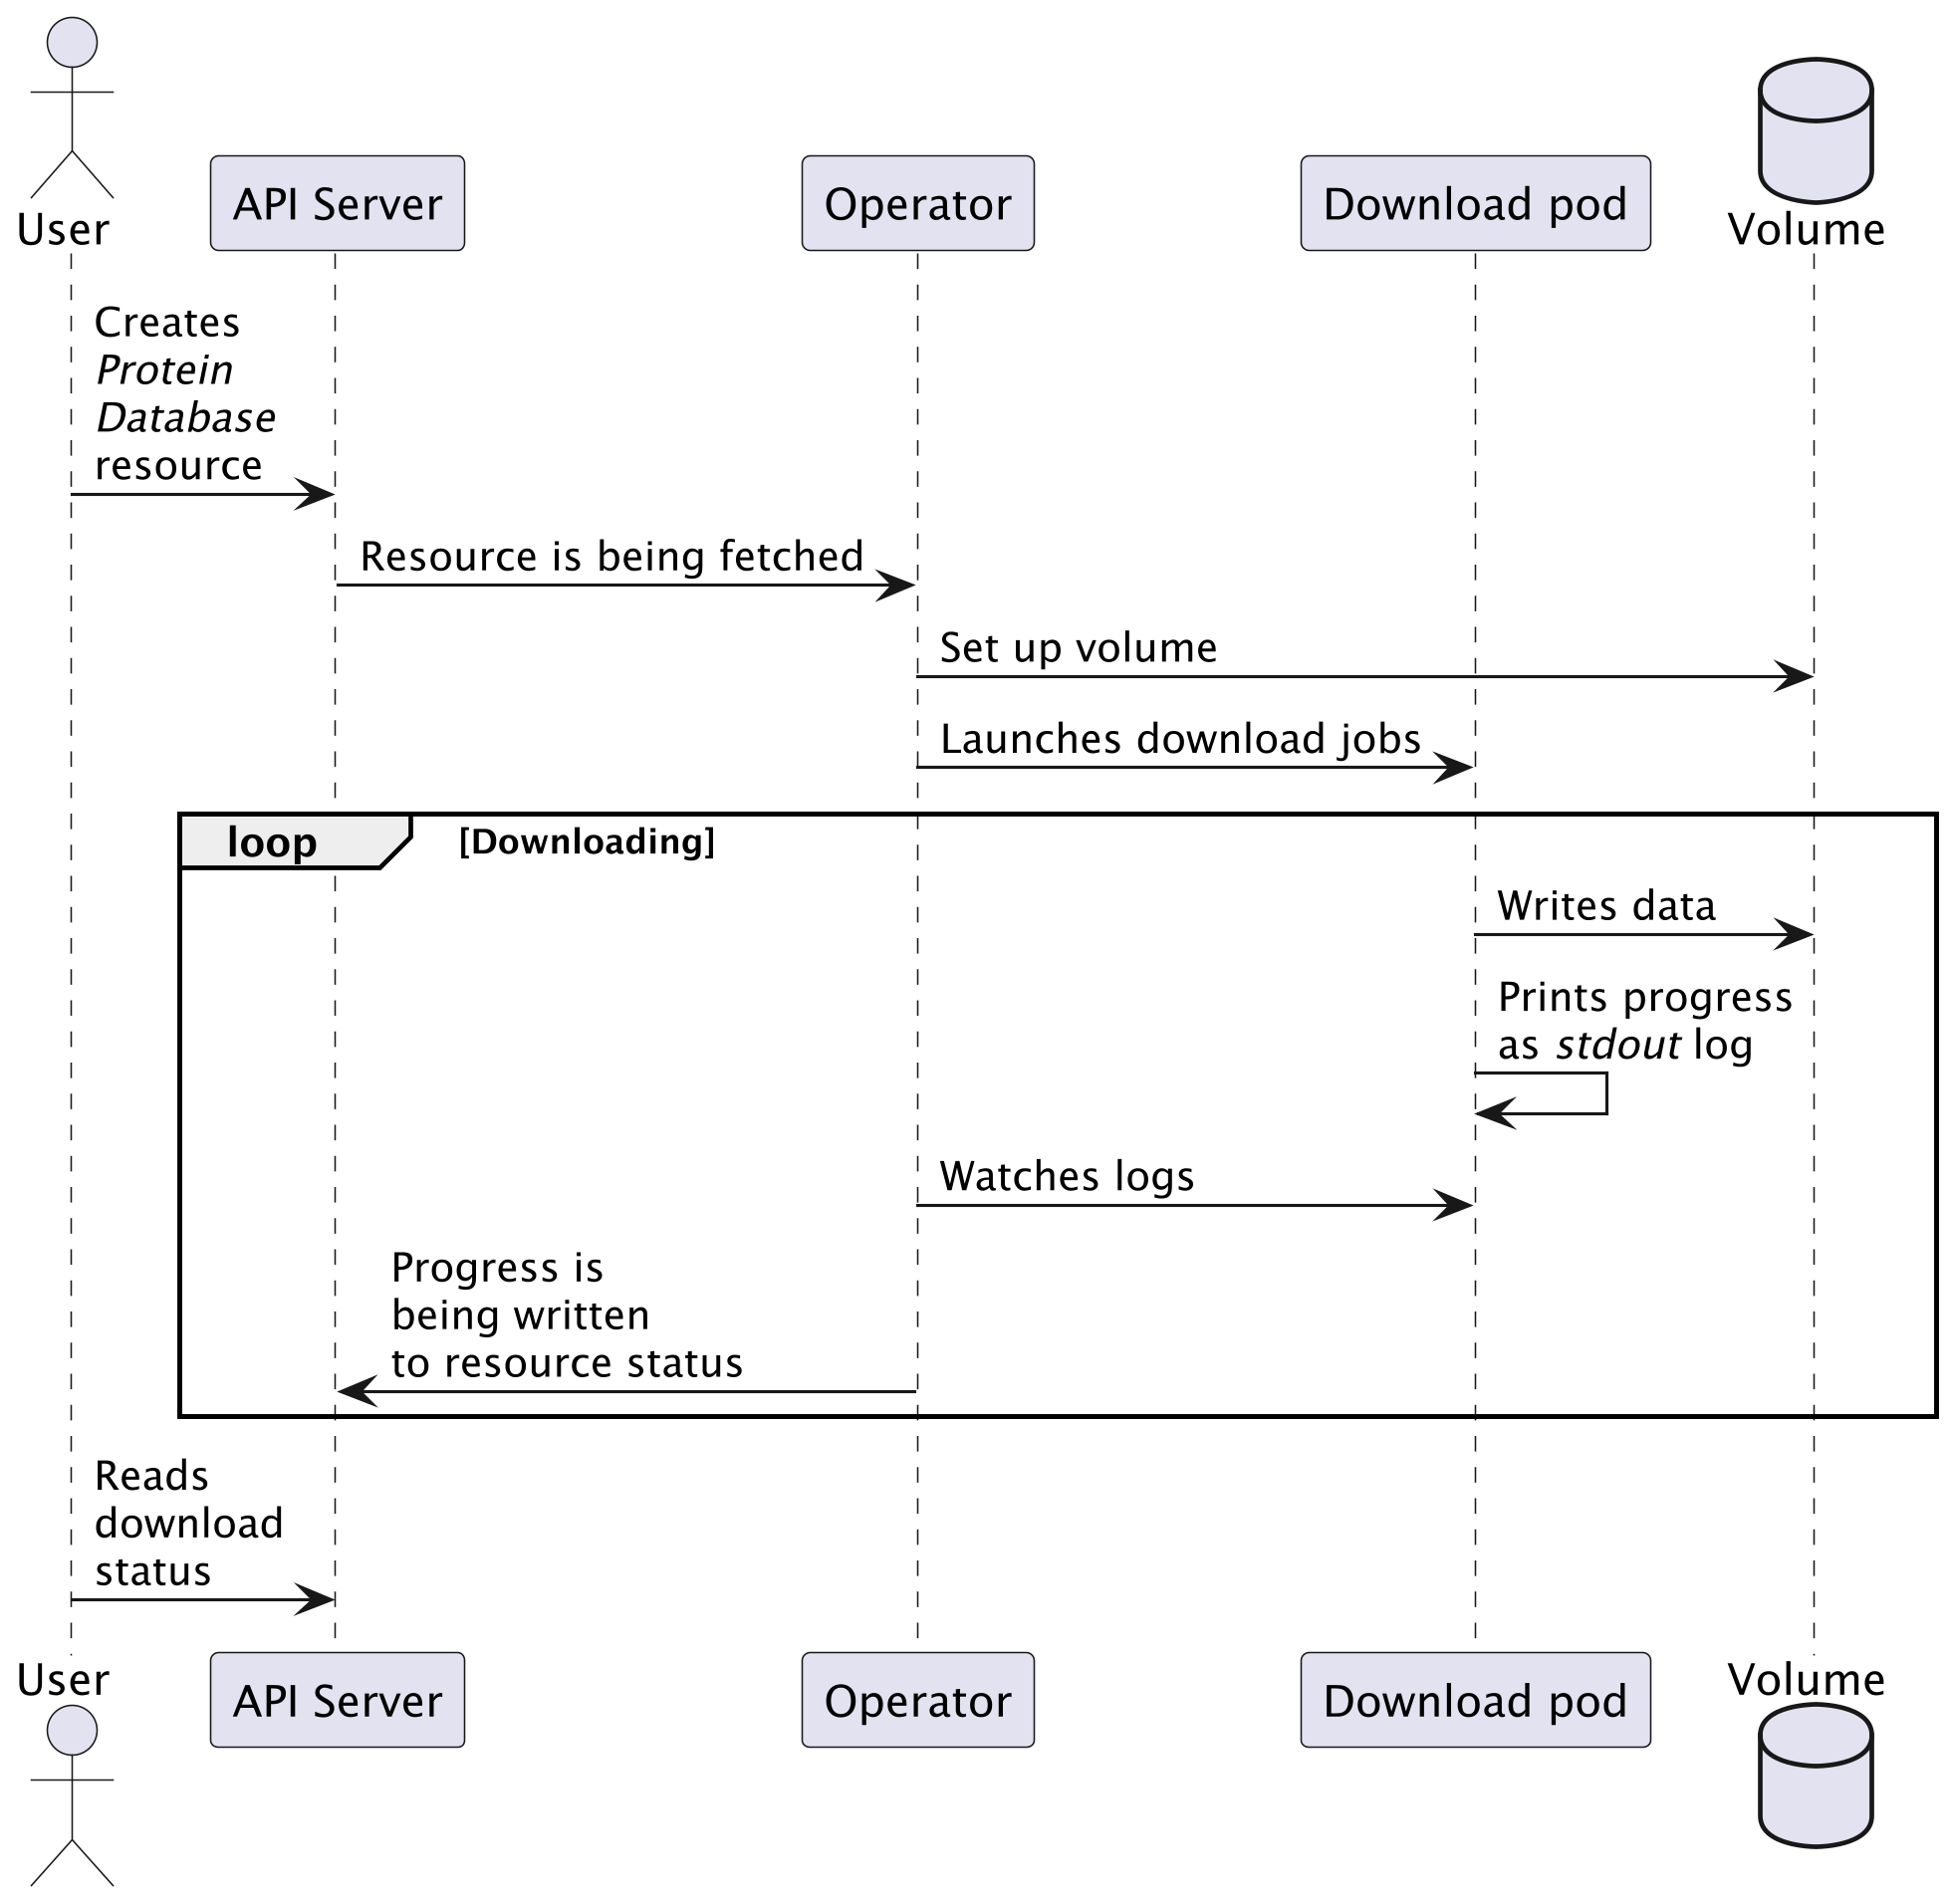
\includegraphics[width=\textwidth]{images/proteindatabase_controller}
    \caption{ProteinDatabase Controller behaviour}
    \label{fig:proteindatabase_controller}
\end{figure}

\begin{figure}[htbp]
    \centering
    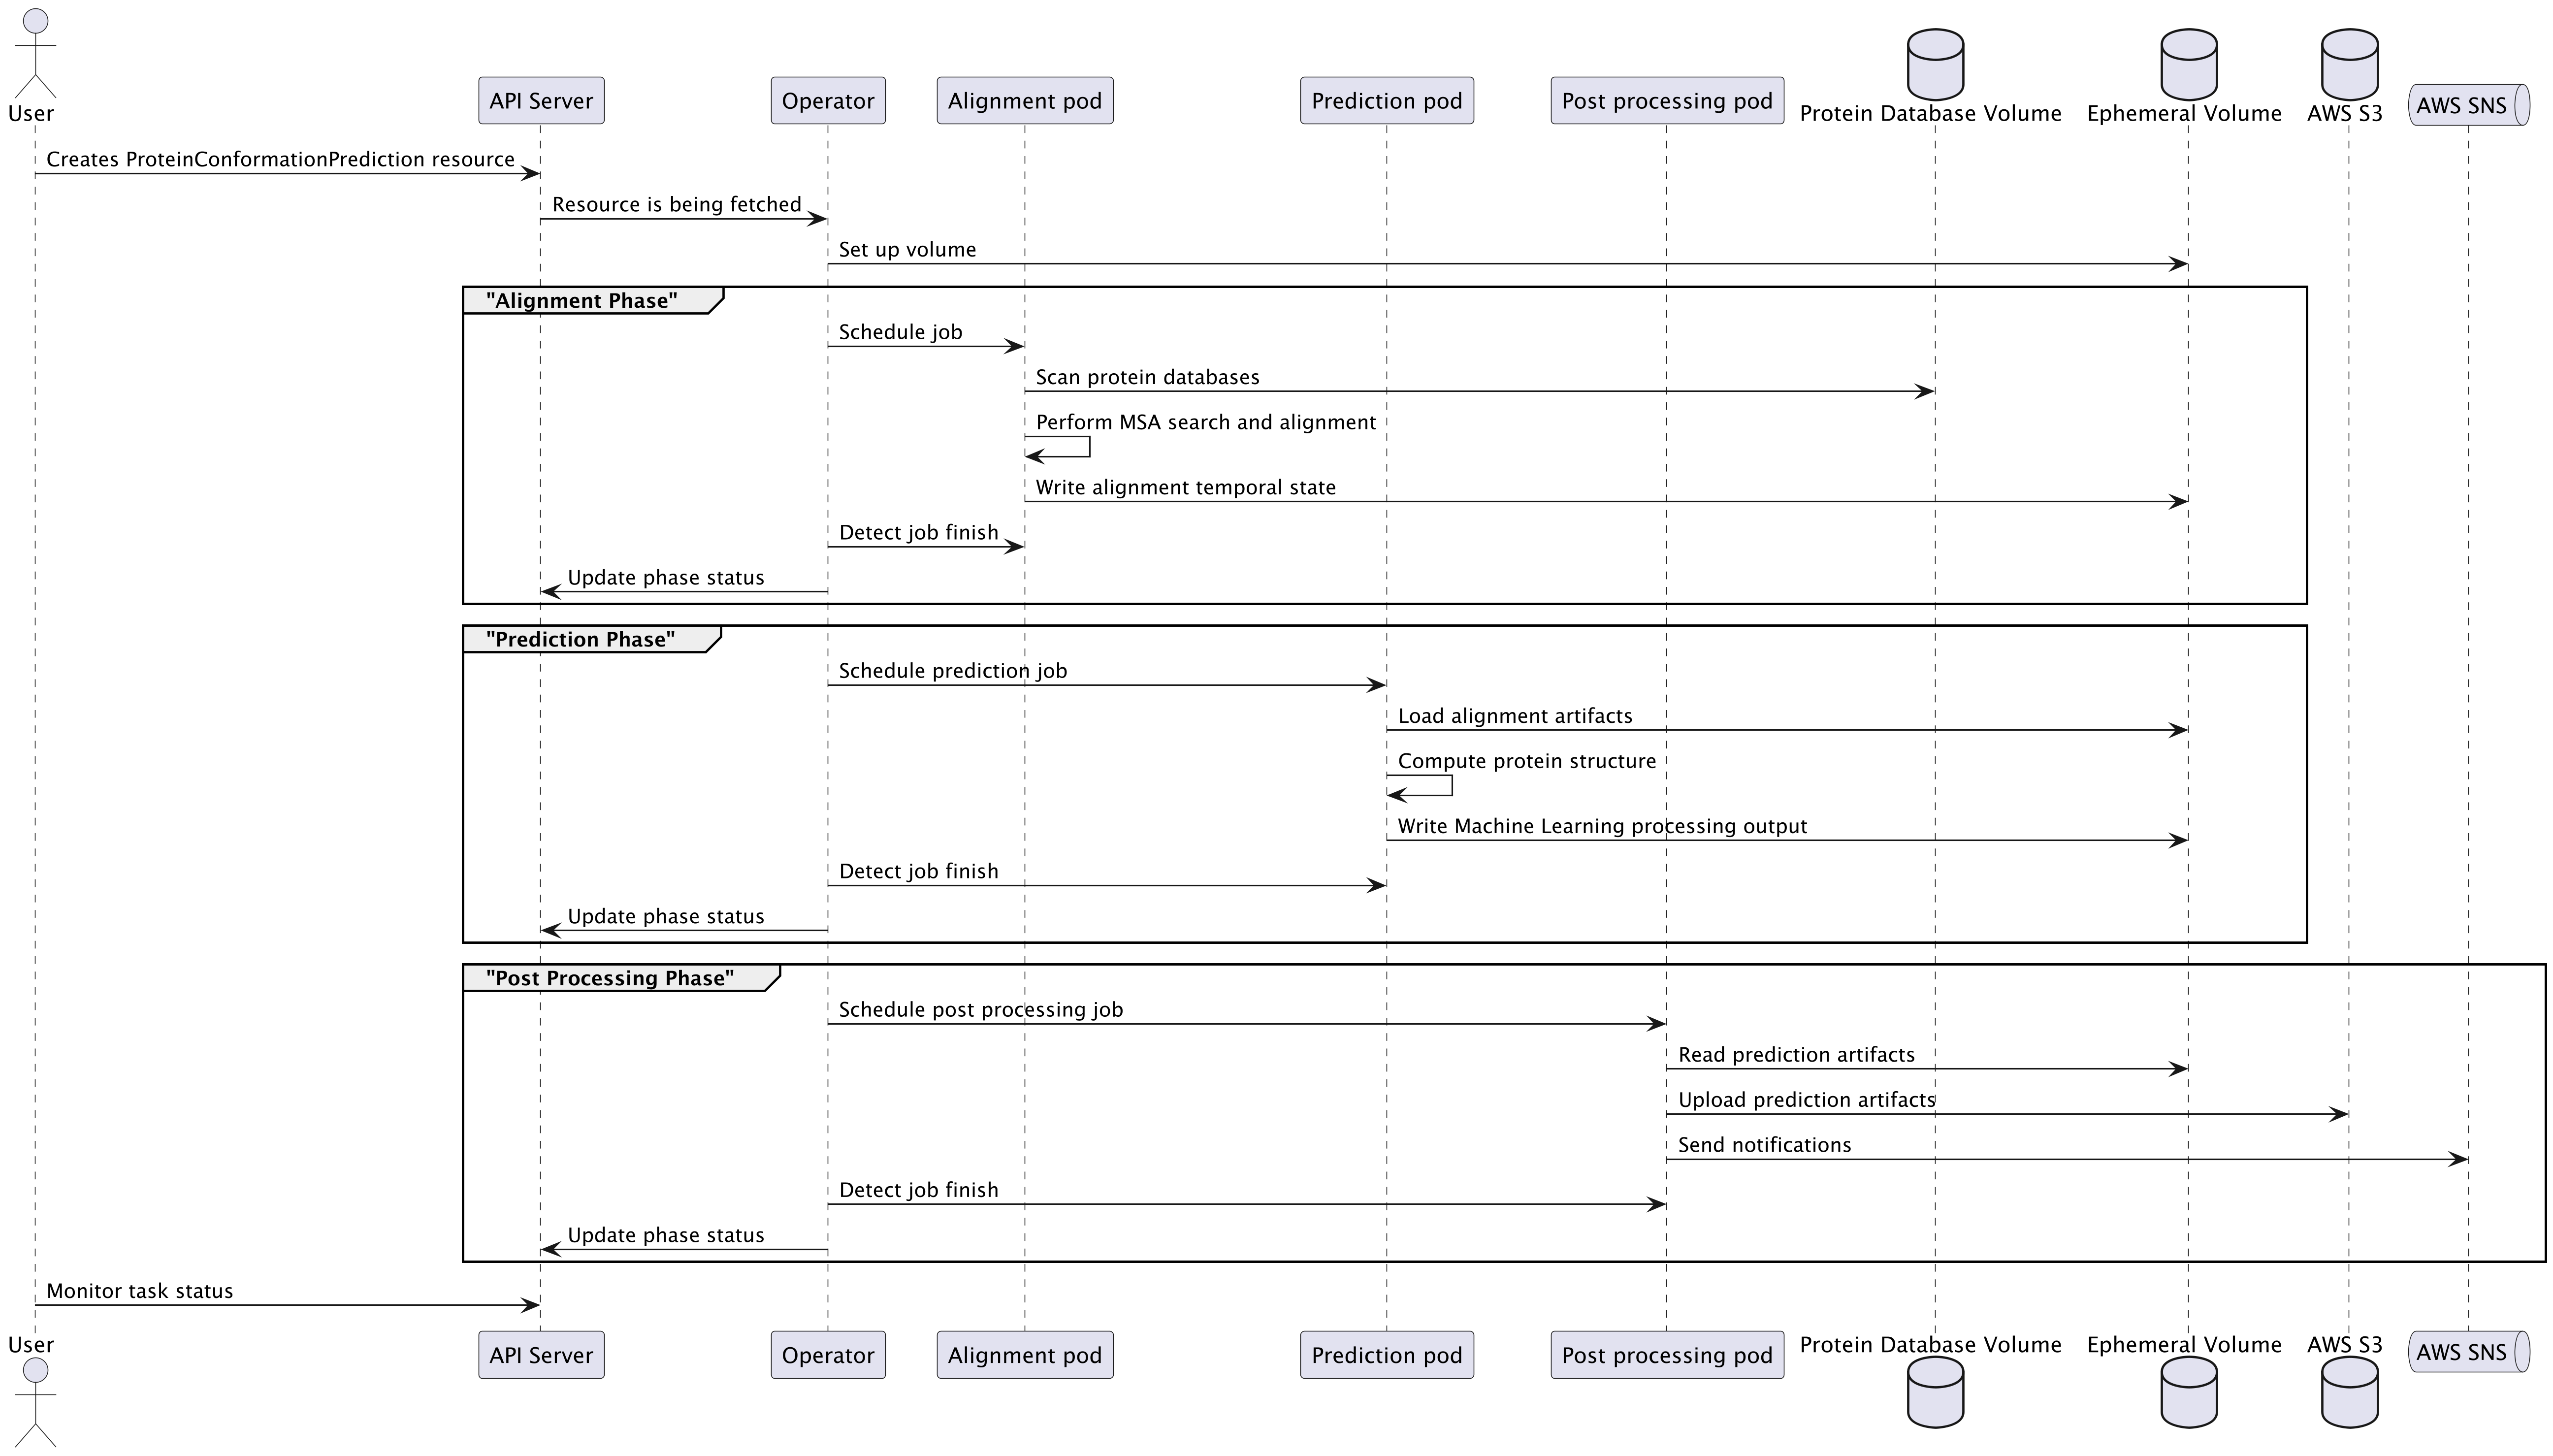
\includegraphics[width=0.9\textwidth]{images/proteinconformationprediction_controller}
    \caption{ProteinConformationPrediction Controller behaviour}
    \label{fig:proteinconformationprediction_controller}
\end{figure}

Drugi kontroler obsługuje zasób \textit{ProteinConformationPrediction}.
Zawiera on logikę obsługującą kolejne trzy fazy predykcji struktury białka.
Logika biznesowa (przedstawiona na diagramie~\ref{fig:proteinconformationprediction_controller}) po wykryciu nowego zasobu realizuje następujace kroki:
\begin{enumerate}
    \item Tworzy nowy PersistentVolumeClaim służący do przechowywania tymczasowych plików programu AlphaFold.
    \item Uruchamia Job, który wykonuje Alignment sekwencji i zapisuje stan do tymczasowego wolumenu.
    Montuje również wolumen zawierający bazy danych białek.
    Program AlphaFold oczekuje podania ustawień startowych (między innymi sekwencji aminokwasów) jako plik w formacie JSON o nazwie \texttt{fold\_input.json}.
    Ten plik jest w tym kroku tworzony za pomocą tak zwanego initContainera~\cite{k8s_init_containers}.
    Treść pliku jest przygotowywana jeszcze w operatorze, po czym jest ona enkodowana do \texttt{base64} i wstrzykiwana do kontenera inicjalizującego przez zmienne środowiskowe.
    Kontener inicjalizujący używa obrazu komponentu managera (opisanego w~\ref{subsec:component-manager}).
    \item Uruchamia Job odpowiadający za predykcję trójwymiarowej struktury białka.
    Kontroler montuje poprzednio używany wolumen, który zawiera stan z poprzedniej fazy.
    Ten Job ma ustawiane nodeAffinity tak, by był schedulowany na węzłach o dużej mocy obliczeniowej GPU.
    \item Uruchamia Job do post processingu.
    Ten krok ładuje artefakty obliczeń i przesyła je do magazynu AWS S3. Odpowiada również za zakolejkowanie powiadomień (np.
    SMS) dla poszczególnych członków zespołu badawczego.
\end{enumerate}

\subsection{Komponent downloader}\label{subsec:component-downloader}
\textit{Repozytorium kodu: \url{https://github.com/kubefold/downloader}}

Komponent \textit{downloader} służy do pobierania jednej wybranej bazy danych białek.
Uruchomienie tego komponentu w kontenerze skutkuje automatycznym rozpoczęciem pobierania.
Kontener oczekuje skonfigurowania następujących zmienncyh środowiskowych:

\begin{itemize}
    \item \texttt{DATASET} - nazwa zbioru danych.
    Dopuszczalne wartości tej zmiennnej są z góry ustalone.
    Są to:
    \subitem \texttt{mgy\_clusters\_2022\_05.fa} - MGY Clusters
    \subitem \texttt{bfd-first\_non\_consensus\_sequences.fasta} - BFD non-consensus sequences
    \subitem \texttt{uniref90\_2022\_05.fa} - UniRef90
    \subitem \texttt{uniprot\_all\_2021\_04.fa} - UniProt
    \subitem \texttt{pdb\_2022\_09\_28\_mmcif\_files.tar} - PDB mmCIF files
    \subitem \texttt{pdb\_seqres\_2022\_09\_28.fasta} - PDB sequence resources
    \subitem \texttt{rnacentral\_active\_seq\_id\_90\_cov\_80\_linclust.fasta} - RNACentral
    \subitem \texttt{nt\_rna\_2023\_02\_23\_clust\_seq\_id\_90\_cov\_80\_rep\_seq.fasta} - NT RNA
    \subitem \texttt{rfam\_14\_9\_clust\_seq\_id\_90\_cov\_80\_rep\_seq.fasta} - RFam
    \item \texttt{DESTINATION} - ścieżka do katalogu wyjściowego.
    \item \texttt{RATE} (opcjonalnie) - limit prędkości pobierania wyrażony w kilobajtach na sekundę.
    Domyślnie proces pobierania nie ma ustawionego górnego limitu.
\end{itemize}.

Wszystkie bazy danych są hostowane w usłudze Google Cloud Storage.
Prawie wszystkie z nich to pliki w formacie \textit{.fasta}~\cite{pearson1988fasta} skompresowane z użyciem algorytmu \textit{ZStandard} (lub krócej \textit{zstd}) od Facebooka~\cite{zstandard}.
Wyjątkiem stanowi plik \texttt{pdb\_2022\_09\_28\_mmcif\_files.tar}, który jest archiwum TAR (również jest skompresowany algorytmem \textit{zstd}).

Komponent pobiera i dekompresuje pliki w tym samym momencie.
Co kilka chwil oddzielny wątek monitoruje progres już pobranych danych wypisując do \texttt{stdout} logline z bieżącym stanem.
Przykładowy logline jest przedstawiony na listingu~\ref{lst:downloader_logline}.
Dzięki temu operator może odczytywać progres pobierania i aktualizować status zasobu \textit{ProteinDatabase}.
Po skończonym sukcesem lub przerwanym w trybie awaryjnym pobieraniu, proces wychodzi logując odpowiedni komunikat do logów oraz zwracając odpowiedni exit code.

\begin{lstlisting}[language=txt,caption={Sample logline from downloader},label={lst:downloader_logline}]
{"dataset":"rnacentral_active_seq_id_90_cov_80_linclust.fasta","level":"info","msg":"Download progress","size":7700349721,"time":"2025-05-17T16:53:52+02:00","total":13860314914,"type":"download","unit":"bytes"}
\end{lstlisting}

\subsection{Komponent managera}\label{subsec:component-manager}
\textit{Repozytorium kodu: \url{https://github.com/kubefold/manager}}

Komponent managera odpowiada za trzy niezależnie od siebie zadania:
\begin{itemize}
    \item konfigurowanie pliku wejściowego \textt{fold\_input.json} dla programu AlphaFold.
    \item wysyłanie artefaktów obliczeń do usługi AWS S3 (o której więcej w sekcji~\ref{subsec:amazon-s3-object-storage}).
    \item kolejkowanie powiadomień za pomocą usługi AWS SNS / AWS End User Messaging (o której więcej w sekcji~\ref{subsec:amazon-sns})
\end{itemize}

Wybór wykonywanej operacji zależy od tego, jakie zmienne środowiskowe zostaną skonfigurowane w kontenerze.
Dla każdej operacji wymagane jest podanie dwóch obowiązkowych zmiennych środowiskowych:
\begin{itemize}
    \item \texttt{INPUT\_PATH} - ścieżka do katalogu danych wejściowych programu AlphaFold
    \item \texttt{OUTPUT\_PATH} - ścieżka do katalogu danych wyjściowych programu AlphaFold
\end{itemize}

W celu zapisu pliku wejściowego \textt{fold\_input.json} należy ustawić zmienną \texttt{ENCODED\_INPUT}, która powinna zawierać zakodowany w \texttt{base64} kod JSON zawierający konfigurację obliczeń.

Z kolei w celu wysłania artefaktów należy ustawić zmienną środowiskową \texttt{BUCKET} na nazwę bucketu usługi S3 (pełna scieżka, wraz w prefiksem \textt{s3:\/\/}).
Aby wysłać powiadomienie za pomocą usługi AWS End User Messaging kontener musi mieć ustawione zmienne \texttt{NOTIFICATION\_PHONES} i \texttt{NOTIFICATION\_MESSAGE}.
Zmienna z numerami telefonów może zawierać więcej niż jednego odbiorcę-w takim przypadku należy podać phone numbers jako listę oddzieloną przecinkami.

Oczywiście w przypadku korzystania z usług AWS powinny zostać skonfigurowane zmienne klienta AWS. Można to zrealizować za pomocą np. zmiennych środowiskowych \texttt{AWS\_ACCESS\_KEY\_ID} i \texttt{AWS\_SECRET\_ACCESS\_KEY}.
Alternatywą jest skonfigurowanie roli AWS IAM, która ma być używana przez kontener i posiada permisje dostępu do poszczególnych usług.